\section{INTRODUCTION}

As a research university, we offer undergraduate students opportunities to work on major research projects, with different students rotating in and out, semester to semester. For those more interested in the applied disciplines (e.g. engineering, journalism, law, business, social work) there are fewer such opportunities. We describe a course design which would give the ``major project" experience in an experiential form, for students in the applied disciplines. We call it multi-semester/multi-cohort, \textbf{MSMC} in this paper.

\begin{figure}[!ht]
  \centering
  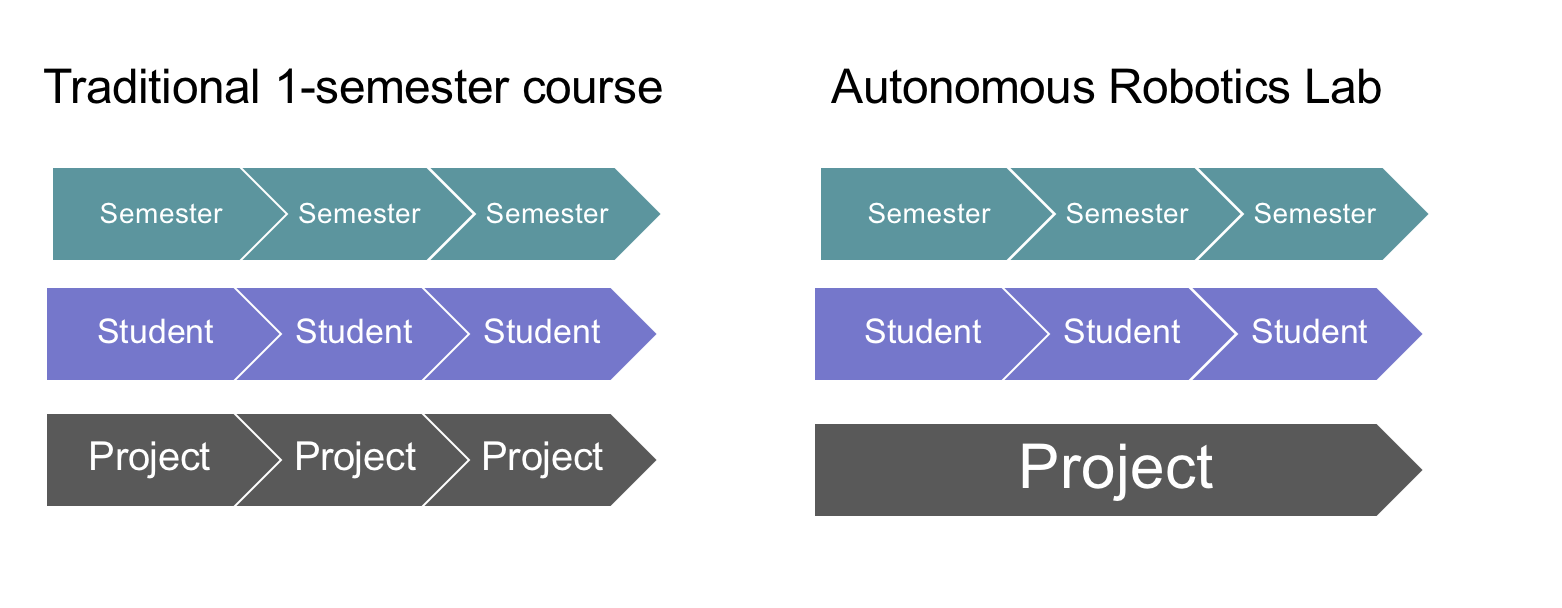
\includegraphics[width=\columnwidth,height=6cm]{diag1}
  \caption{Multi Semester/Multi Cohort structure}
  \label{fig:diag1}
\end{figure}

``Multi-semester'' because the objective will not achieved in one semester, and ``multi-cohort'' because the set of students working on it changes from semester to semester. This approach has many benefits, but poses some obvious challenges which will be addressed below.

We are inspired by the idea of a \textbf{BHAG} (\textit{Big Hairy Audacious Goal}), conceptualized in \cite{Collins}. Collins and Porras describe this mouthful term as follows:

\begin{quote}
``We found in our research that visionary companies often use bold missions --- BHAGs, shorthand for Big, Hairy, Audacious Goals --- as a powerful way to stimulate progress.... A true BHAG is clear and compelling, serves as a unifying focal point of effort, and acts as a catalyst for team spirit. It has a clear finish line, so the organization can know when it has achieved the [goal] A BHAG engages people --- it reaches out and grabs them. It is tangible, energizing, highly focused.\cite{Collins}''
\end{quote}

Obviously our MSMC structure for the course is a variant of well established ``Project-Based Learning'' pedagogy\cite{projects}, and our ``BHAG'' just another name for the ``driving question'' defined in \cite{blumenfeld}. We are attracted to the idea of a BHAG because it clearly implies a driving question which almost by definition cannot be completed in one semester, thereby supporting the idea of a multi-semester course structure.

For our course, our BHAG is ``Campus Rover'', a mobile, wheeled, robot that can travel both indoors and outdoors on a campus to deliver packages, navigating from from an office in one building to an office in another building. Over the course of the preceding two semesters, we have made changes and refinements in the program. We are now in our third semester. This paper captures our experience and lessons up to now, both what worked and what can be improved.

